\documentclass{article}
\usepackage[italian]{babel}
\usepackage[utf8]{inputenc}
\usepackage{fancyhdr}
\usepackage{tikz}
\usepackage{amsmath}
\usepackage{amssymb}
\usepackage{amsthm}
\usepackage{amsfonts}
\usepackage{color}
\usepackage{circuitikz}
\usepackage[margin=2cm]{geometry}
\usepackage[scientific-notation=true]{siunitx}
\usepackage{titlesec}
\usepackage{graphics}

\titleformat{\paragraph}
  {\normalfont\normalsize\bfseries}{\theparagraph}{1em}{}
\titlespacing*{\paragraph}
  {0pt}{3.25ex plus 1ex minus .2ex}{1.5ex plus .2ex}

\title{Analisi di un circuito RLC serie in regime sinusoidale}
\date{18/05/2022}
\author{Bertasi Leonardo mat. 970881, Perniola Davide mat. 989409}
\begin{document}
\maketitle
\section{Abstract} 
In questa esperienza si è analizzato il comportamento di un circuito RLC serie in regime sinusoidale. Misurando le tensioni ai capi delle componenti è stato possibile
verificare la differenza di comportamento tra di esse. A tale scopo sono sati acquisiti i dati relativi a tre frequenze significative in un intorno della frequenza di risonanza attesa $f_0=(7351\pm68)Hz$.
Inoltre si è studiato l'andamento dell'ampiezza e della fase delle tensioni ai capi delle componenti in funzione della frequenza. Da questa analisi si è ricavto il valore delle frequenza di risonanza sperimentale $f_0s=(7562\pm5)Hz$.
L'incompatibilità tra i due valori è spiegata dalla presenza di errori sistematici nell'acquisizione non valutabili. 


\section{Introduzione} 
Un circuito RLC serie consiste in una resistenza, una induttanza e un condensatore posti in serie. Applicando ai capi del ciruito una differenza di potenziale sinusoidale $V_{0}\cos{wt} $ ci si aspetta di osservare un preciso andamento, anch'esso sinusoidale,
 ai capi di ognuno degli elementi circuitali. L'unica corrente che scorre nel circuito segue la relazione(si veda appendice) 
\begin{equation}
  i(t)=\frac{V_{0}}{\sqrt{R^2+(wL-\frac{1}{wC})^2}}\cos{[wt+(\arctan{\frac{1-w^2LC}{wRC}})]}
\end{equation}
Utilizzando la (1) si possono scrivere gli andamenti teorici della tensione ai capi della resistenza
\begin{equation}
 V_{R}(t)= \frac{V_{0}R}{\sqrt{R^2+(wL-\frac{1}{wC})^2}}\cos{[wt+(\arctan{\frac{1-w^2LC}{wRC}})]}
\end{equation}

dell'induttanza
\begin{equation}
  V_{L}(t)=\frac{V_{0}wL}{\sqrt{R^2+(wL-\frac{1}{wC})^2}}\cos{[wt+(\arctan{\frac{1-w^2LC}{wRC}})+\frac{\pi}{2}]}
\end{equation}

del condensatore
\begin{equation}
  V_{C}(t)=\frac{(\frac{V_{0}}{wC})}{\sqrt{R^2+(wL-\frac{1}{wC})^2}}\cos{[wt+(\arctan{\frac{1-w^2LC}{wRC}})-\frac{\pi}{2}]}
\end{equation} 

Ricordando che la pulsazione di risonanza per un circuito RLC è $w_0=\frac{1}{\sqrt{LC}}$ e che il modulo della corrente che scorre nel circuito alla frequenza di risonanza corrispondente $f_0$ è massimo, alla frequenza di risonanza ci si aspetta di 
osservare $V_R(t)$ in fase con la sorgente e massimo in ampiezza, $V_L(t)$ in anticipo di $\frac{\pi}{2}$ rispetto alla sorgente e $V_C(t)$ in ritardo di $\frac{\pi}{2}$ rispetto alla sorgente e della stessa ampiezza di  $V_C(t)$. \\
Si può esplicitare la dipendeza dell'ampiezza massima e della fase delle tensioni in funzione della pulsazione $w$ semplicemente considerando il modulo delle ampiezze e della fase alle diverse tensioni. Ad esempio risulta

\begin{equation}
 A_R(w) =\frac{V_{0}R}{\sqrt{R^2+(wL-\frac{1}{wC})^2}} \qquad \Phi_R(w)=\arctan{\frac{1-w^2LC}{wRC}}
\end{equation}






In generale si prevede
un aumento dell'ampiezza di $V_L$ e una diminuzione dell'ampiezza di $V_C$ proporzionale ad $w$, mentre per $V_R$ l'ampiezza aumenta fino al massimo in corrispondenza di $f_0$ per poi decrescere sempre proporzionalmente a $w$. \\Per quanto riguarda la fase inoltre, notando come 
\begin{equation}
  \lim_{w \to + \infty}\arctan{\frac{1-w^2LC}{wRC}} = -\frac{\pi}{2}
\end{equation}
è chiaro aspettarsi, aumentando $w$, la decrescita della fase della tensione ai capi di ogni componente e lo stabilizzarsi di quest'ultima a 0 per $V_L(t)$, $-\frac{\pi}{2}$ per $V_R(t)$ e $-\pi$ per $V_C(t)$.





\section{Apparato sperimentale e svolgimento}
\begin{figure}[h!]
  \begin{center}
    \begin{circuitikz}[]
      \draw (0,0)
      to[vsourcesin=$V_S$] (0,2) % The voltage source
      to[R=$R_I$] (0,4)
      

      to[R=$R$] (2,4) % The resistor
      to[R=$R_L$] (4,4)
      
      to[L=$L$] (4,0)
      to[short] (4,0)
      to[C=$C$] (0,0)
      to[short] (0,0);

    \end{circuitikz}
    \caption{\textit{Schema del circuito realizzato.}}
  \end{center}
\end{figure}
Il circuito RLC è stato realizzato sulla breadboard della scheda di acquisizione NI ELVIS II ed è schematizzato in Figura 1. Esso è alimentato dal function generator di ELVIS di resistenza interna $R_I=50\Omega$ come da specifiche della scheda. Nel ciruito sono presenti, disposti in serie, 
una induttanza $L=(10.3\pm0.1)mH$, un condensatore $C=(45.5\pm0.4)nF$ una resistenza $R=(330.0\pm0.3)\Omega$ e una resistenza $R_L=(34.5\pm0.1)\Omega$ che tiene conto della resistenza interna dell'induttore. Tutti i valori delle componenti riportati sono stati misurati utilizzando il multimetro digitale di ELVIS.
Per verificare il corretto funzionamento delle componenti è stato utilizzato un oscilloscopio, osservando così il comportamento del ciruito in un intorno della frequenza di risonanza attesa. Successivamente servendosi di un programma scritto in LabView sono state acquisite le misure delle tensioni ai capi del generatore, resistenza, induttanza e consensatore relative ad una frequenza $f_m=4000Hz$, una $f_0=7351Hz$ e  $f_M=10000Hz$ in modo tale da evidenziare le differenze del comportamento del circuito all'interno di un ampio range di frequenze e in particolare alla frequenza di risonanza.
Per far questo si è usata una frequenza di acquisizione di $50000Hz$ nel primo caso, di $100000Hz$ nel secondo e di $150000Hz$ nel terzo, affinchè questa si mantenga ad un valore di almeno dieci volte quello della frquenza del segnale acquisito.
Infine si è studiato l'andamento della fase e dell'ampiezza della tensione ai capi delle componenti in funzione della frequenza. Per far ciò si è impostato nel funcion generetor uno \textit{sweep} sulla frequenza nel range compreso tra $3000Hz$ e $13000Hz$, con \textit{step} di $100 Hz$ e \textit{step interval} di $1000ms$. 

\section{Risultati e discussione}
\subsection{Tensione in funzione del tempo}
\begin{figure}[]
  \centering
  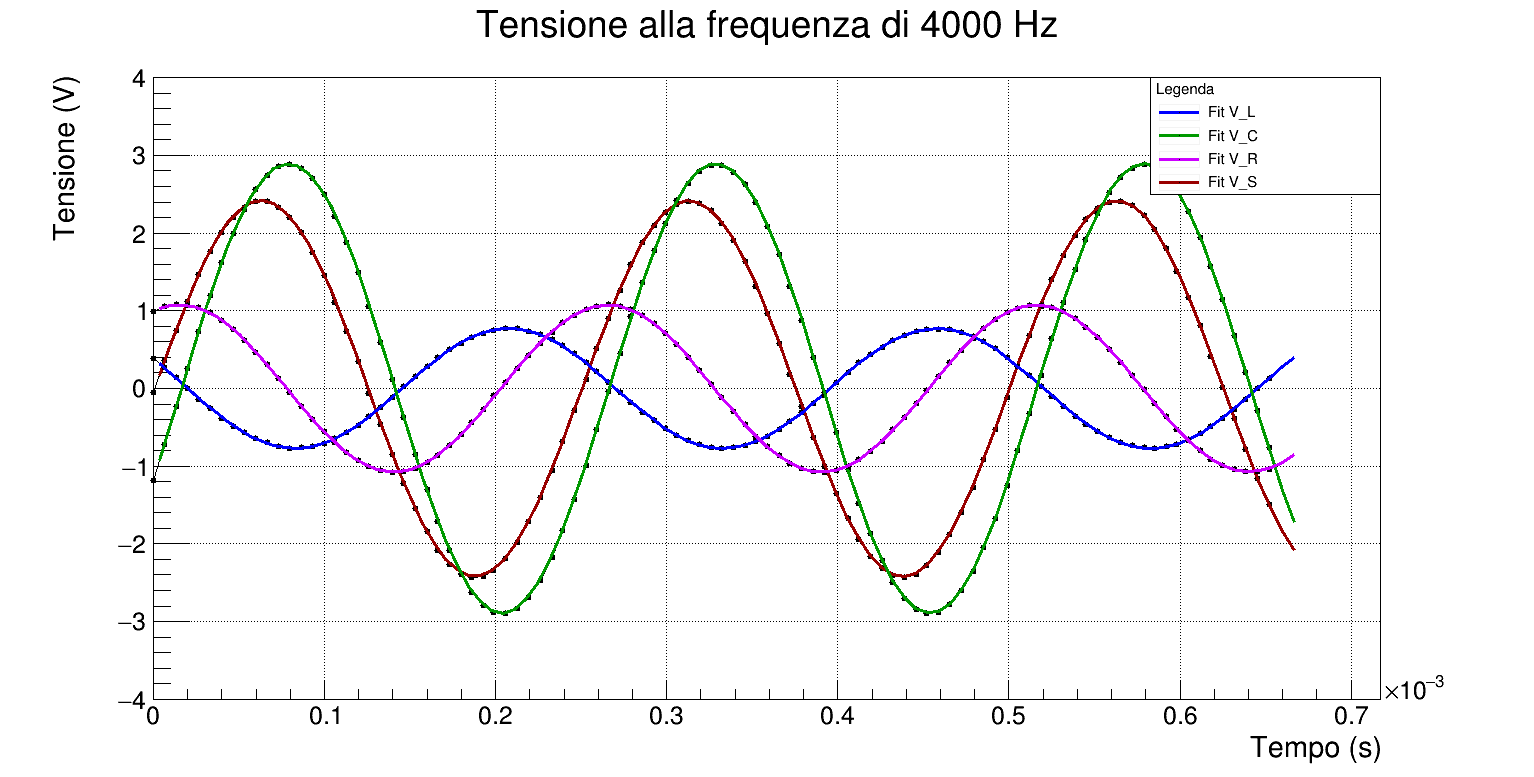
\includegraphics[scale=0.27]{FitFMin.png}
  \qquad
  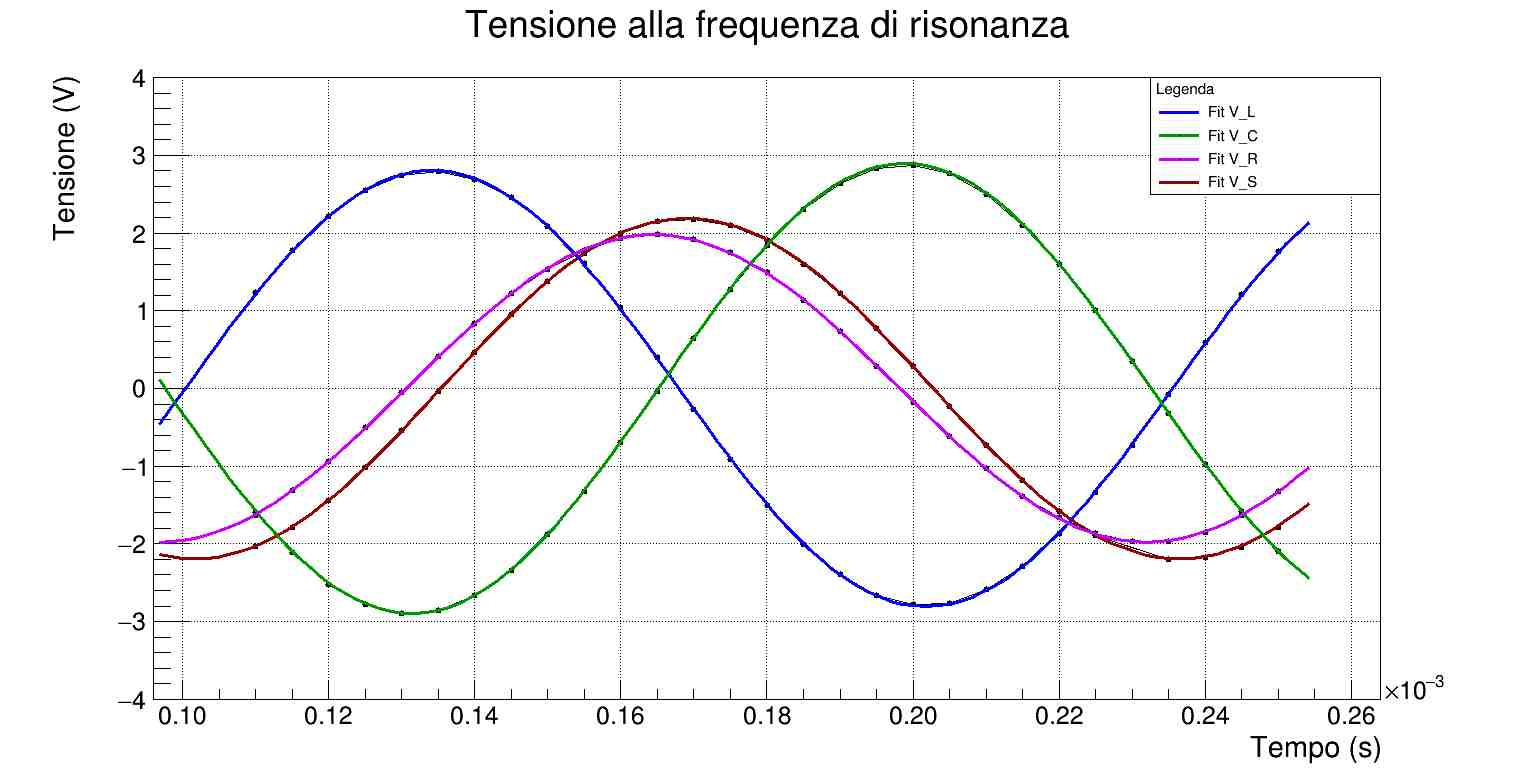
\includegraphics[scale=0.27]{FitF0.jpg}
  \qquad
  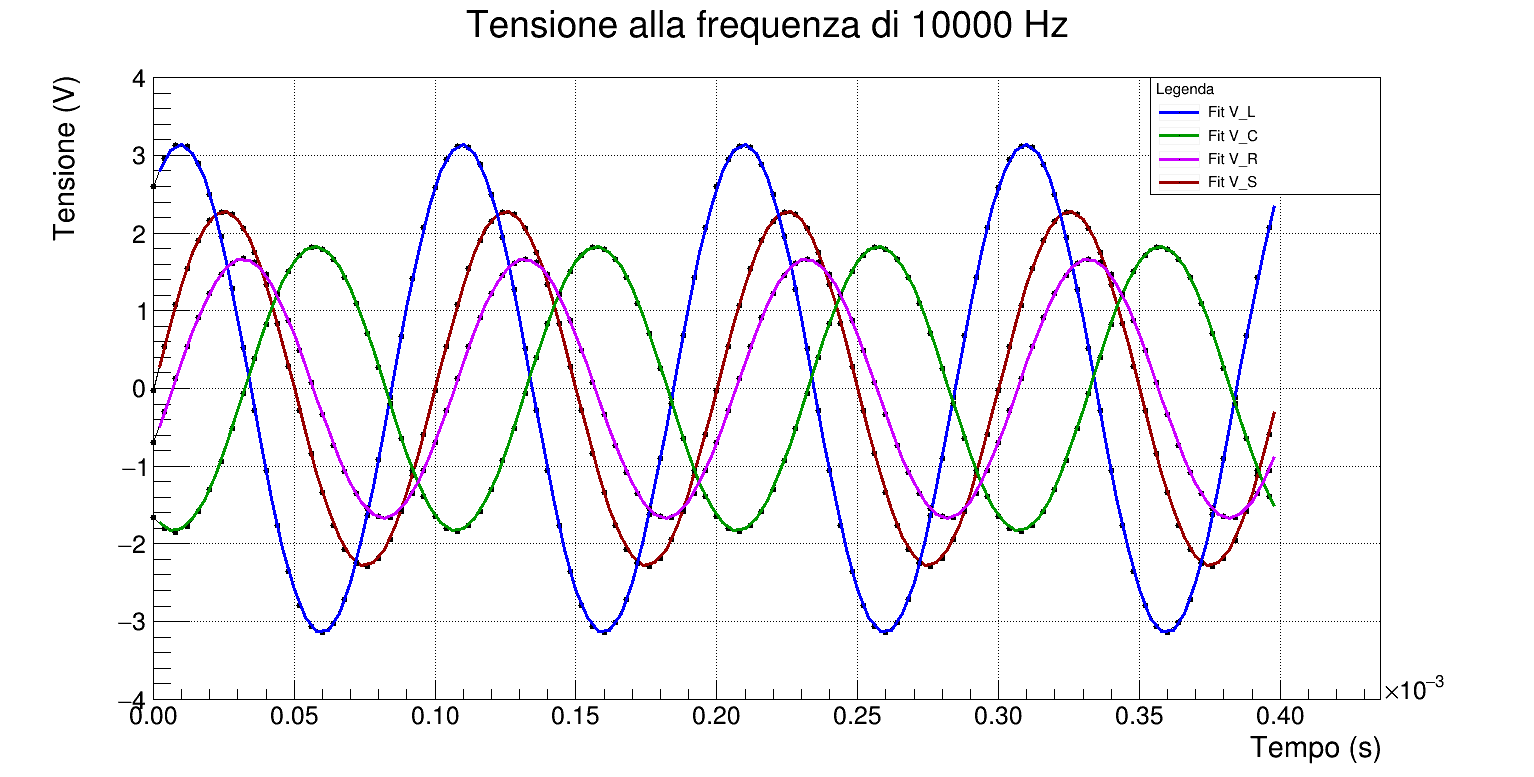
\includegraphics[scale=0.27]{FitFMag.png}
  \caption{\textit{Confronto tra le tensioni in funzione del tempo ai capi degli elementi circuitali relativi alle tre diverse frequenze utilizzate. In alto $f_m$,in mezzo $f_0$ e in basso $f_M$. Sull'asse x il tempo è nel formato $(10^{-3}s)$, come scritto in basso a destra nel grafico. }}
\end{figure}
In Figura 2 sono riportate le tensioni in funzione del tempo ai capi di ogni elemento del circuito per i tre valori di frequenza scelti. Si può subito notare che gli andamenti teorici (descritti nell'introduzione) sono rispettati: considerando $V_L$ si vede come la sua ampiezza cresca 
nei grafici a frequenza di risonanza e $10000Hz$ rispetto al grafico a $4000Hz$. Al contrario per $V_C$ l'ampiezza decresce una volta superata $f_0$, mentre $V_R$ come previsto cresce fino a raggiungere un massimo a quella frequenza per poi tornare a diminuire. \\ Osseravando 
il grafico alla frequenza di risonanza si nota come $V_L$ e $V_C$ siano sfasati di circa $-\frac{\pi}{2}$ e $\frac{\pi}{2}$ rispettivamente e di come $V_R$ e $V_S$ non siano perfettamente in fase. 
Quest'ultimo sfasamento denota una differenza tra la frequenza di risonanza attesa e quella sperimentale. I grafici sono stati ottenuti effettuando i fit delle equazioni (2),(3),(4) ai dati sperimentali. L'incertezza sulla tensione è stata ottenuta analizzando il rumore del function generator, ovvero la deviazione standard di un campione di misure relative a un semiperiodo di un'onda quadra.
In Tabella 1 sono riporati i risultati numerici dei $\tilde{\chi}^2$ ottenuti dai fit. I valori risultano relativamente grandi rispetto al valore ottimale 1 in quanto l'incertezza totale sulla tensione è probabilmente sottostimata. 

  \begin{table}[h!]
    \centering
   \mbox{%
  \begin{tabular}{|c|c|c|c|c|}
  
  \hline
  $\tilde{\chi}^2$ & $V_S$ & $V_R$ & $V_C$ & $V_L$ \\
  \hline
  
  $4000Hz$ & 25.2 & 3.02 & 30.6 & 5.34\\
  $7351Hz$ & 9.68 &8.31& 15.7& 15.6\\
  $10000Hz$ & 15.3& 4.49 &16.5&7.01 \\
  \hline
  \end{tabular}
   }
   \caption{\textit{Valori del $\tilde{\chi}^2$ per la tensione di ciascuna componente nei tre casi analizzati}}
\end{table}

\subsection{Analisi dell'ampiezza}
\begin{figure}[h]
  \centering
  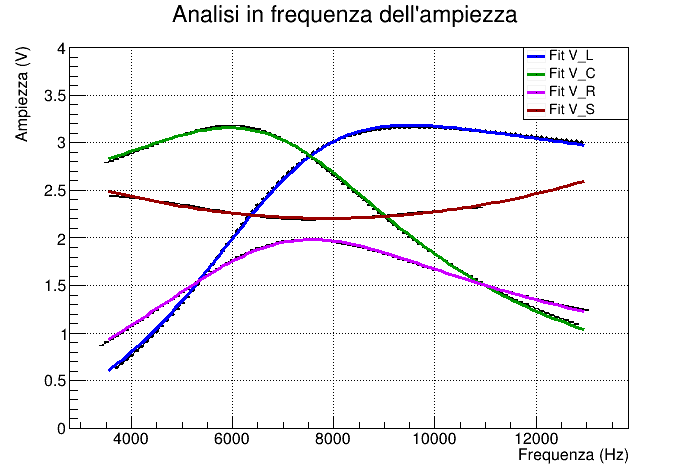
\includegraphics[scale=0.45]{AmpFreq.png}
  \caption{\textit{Ampiezza massima della tensione in funzione della frequenza per ogni componente del circuito.}}

\end{figure}
Il grafico in Figura 3 permette di osservare contemporaneamente gli andamenti dell'ampiezza massima della tensione di ciasciuna componente in base alla frequenza. Si può notare che le curve di $V_L$ e $V_C$ verificano la tendenza riscontrata nell'analisi della tensione in funzione del tempo. Infatti la prima cresce fino a un massimo poco dopo $f_0$ e la seconda, successivamente a un massimo poco prima di $f_0$, descresce.
\`E importante osservare come l'ampiezza di $V_S$ non rimanga costante ma abbia un minimo intorno a $f_0$. Al contrario $V_R$ ha un massimo in un intorno della frequenza di risonanza attesa. Questo conferma quanto detto nel paragrafo precedente: è possibile ricavare un valore sperimentale per la frequenza di risonanza differente da $f_0$.
Questo valore è stato calcolato in corrispondenza del massimo dell'ampiezza di $V_R$ e risulta $f_0s=(7562\pm5)Hz$. Anche in questo caso l'errore sull'ampiezza è un errore casuale ottenuto da un campione di dati ricavato misurando l'ampiezza a frequenza fissata. 
Anche in questo caso i valori del $\tilde{\chi}^2$ riportati in Tabella 2 risultano relativamente elevati a causa di una probabile sottostima dell'incertezza totale. 


\begin{table}[h!]
  \centering
 \mbox{%
\begin{tabular}{|c|c|c|c|}

\hline
$\tilde{\chi}^2$ & $V_R$ & $V_C$ & $V_L$  \\
\hline

Ampiezza & 11.2 & 30.7 & 25.12 \\
Fase & 15.7 & 6.20& 5.99\\
\hline
\end{tabular}
 }
 \caption{\textit{Valori del $\tilde{\chi}^2$ per la tensione di ciascuna componente per il fit in frequenza}}
\end{table}

\subsection{Analisi della fase}
\begin{figure}[h]
  \centering
  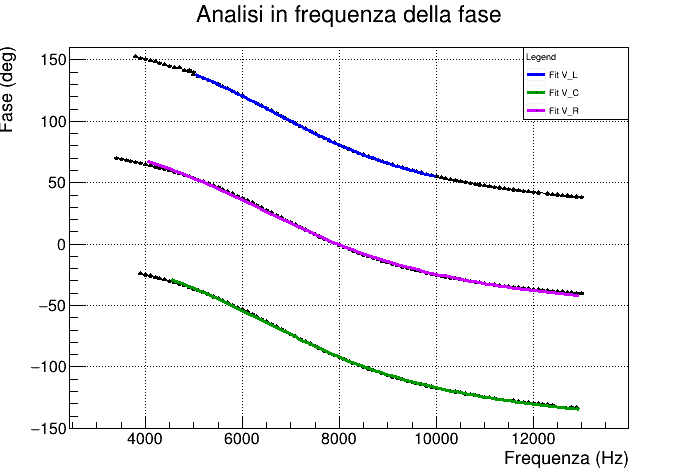
\includegraphics[scale=0.45]{FaseFreq2.png}
  \caption{\textit{Fase della tensione in funzione della frequenza per ogni componente del circuito.}}
\end{figure}
Dal grafico in Figura 4 è possibile verificare il comportamento previsto nella (6). Infatti si osserva come la fase di $V_L$ tenda a 0, quella di $V_R$ tenda a $-\frac{\pi}{2}$ e quella di $V_C$ tenda a $-\pi$ all'aumentare della frequenza. 
Analizzando i dati si evince che la curva di $V_R$ raggiunge il valore 0 in un intorno di $f_0s$. Quest'ultimo risultato può essere stato condizionato da un errore sistematico della schede ELVIS II durante il campionamento:
i segnali dei diversi canali di acqusizione vengono misurati sequenzialmente e pertanto l'ultimo canale acquisirà con un ritardo $\Delta t$ rispetto al primo. 
In riferimento alla Tabella 3  valgono le stesse considerazione sull'incertezze del paragrafo precedente. 
\section{Conclusioni}
L'esperimento ha fornito risultati contrastanti: sebbene il comporatmento atteso del circuito ha trovato buon riscontro nel fit dei dati sperimentali alle curve teoriche, l'analisi in frequenza ha evidenziato una significativa differenza
tra $f_0=(7351\pm68)Hz$ e  $f_0s=(7562\pm5)Hz$. Questo ad esempio si traduce in uno sfasamento tra $V_S$ e $V_R$ a $f_0$ come si nota in Figura 2. 
\`E possibile ipotizzare che questa discordanza si dovuta ad alcuni effetti sisetmatici dovuti alla scelta delle componenti del circuito e alla scheda ELVIS. Infatti l'utilizzo di una resistenza $R=(330.0\pm0.3)\Omega$ di valore comparabile con quello della resistenza interna del function generator $R_I=50\Omega$
può aver condizionato in maniera non trascurabile le misure di $V_R$. Inoltre la scheda di acqusizione riceve i segnali dei diversi canali sequenzialmente ad intervalli di $\Delta t$, fattore che può aver determinato un ulteriore errore sistematico per le misurazioni.


\end{document}
